Um die grossen Datenmengen, von über 1000 Datenpunkten, die für ein robustes ML aus \ref{sec:DB} benötigt werden, liefern zu können, muss die Messung teure menschliche Arbeitszeit drastisch reduzieren. Die Vorstudien in \ref{zweitFeldVer} erforderten rund 9 Stunden Arbeitszeit und hätten etwa 50 LWC-Tapes und 6 LWC-Denoth-Datenpunkte liefern können.

Ein grosser Vorteil des Tapes ist die feine örtliche Auflösung im zehntel Millimeter Bereich in der Messregion von 20 x 20 mm. Um diese feine Auflösung zu nutzen, ist es spannend, Messungen durch die Höhe der Schneedecke durchzuführen.

\begin{itemize}
\item Eine Möglichkeit (siehe Abbildung {fig:AutMess}) besteht darin, dass der Feldforscher mit einer Bohrmaschine ein Loch in den Schnee bohrt. Dann kann das Messsystem in das Loch herabgelassen werden und kontinuierlich Messungen durchführen, während es abgesenkt wird. Mit dieser Anordnung wird nicht mehr in der Horizontalen gemessen, sondern in der Vertikalen. Das wird eine umfassendere Aussage über eine Schneedecke liefern.

\item Den Anpressdruck seitlich aus zu üben ist schwierig. Die Schwerkraft funktioniert nicht direkt. Elastomere sind bei tiefen Temperaturen schwer einzuschätzen. Der Einsatz eines Elektromotors ist möglich, jedoch etwas umständlich aufgrund der Notwendigkeit einer Batterie. Eine Blattfeder oder eine Kompressionsfeder stellen vielversprechende Alternativen dar. Ein pneumatisches System bietet in der Wirkung Vorteile, ist jedoch in der Umsetzung anspruchsvoll.



\item Die flache Geometrie des harten XPS-Schaums kann durch eine Kugel oder einen Kegel ersetzt werden, so kann eine andere Druckkraft erreicht werden.


\item Das Tape kann auf eine Membran geklebt werden, die pneumatisch aufgeblasen wird und so an den Schnee angedrückt wird.

\item Zwischen dem Tape und dem Gewicht kann ein flexibler Schaumstoff eingesetzt werden, so kann sich das Tape an die Unregelmässigkeit des Schnees besser anpassen.

\item Um eine hohe Anpassbarkeit des steifen Tapes an den Schnee zu verbessern, kann das Tape in kleinere Stücke geschnitten werden. So kann sich der elastische Träger des Tapes effektiv an den Schnee anpassen.

\item Es ist auch möglich, dass ein vollautomatisiertes Messsystem über den Sommer an strategisch gewählten Orten aufgebaut wird und dann eingeschneit wird. Hier besteht die Schwierigkeit, an genügend ungetesteten guten Schnee zu gelangen, um eine feine zeitliche Auflösung zu ermöglichen. Mit der vierten Iteration konnte gezeigt werden, dass ein Messung an dem selben Schnee wiederholt werden kann.


\item Ein weiteres Konzept ist, dass das Messsystem von einem Helikopter aus abgeworfen wird. Durch die kinetische Energie schlägt das Messsystem dann durch die Schneedecke. In einer zweiten Phase wird das Tape an den Schnee angepresst und die Daten drahtlos an die Datenbank aus Kapitel \ref{sec:DB} übermittelt.

\end{itemize}

\begin{figure}
    \centering
    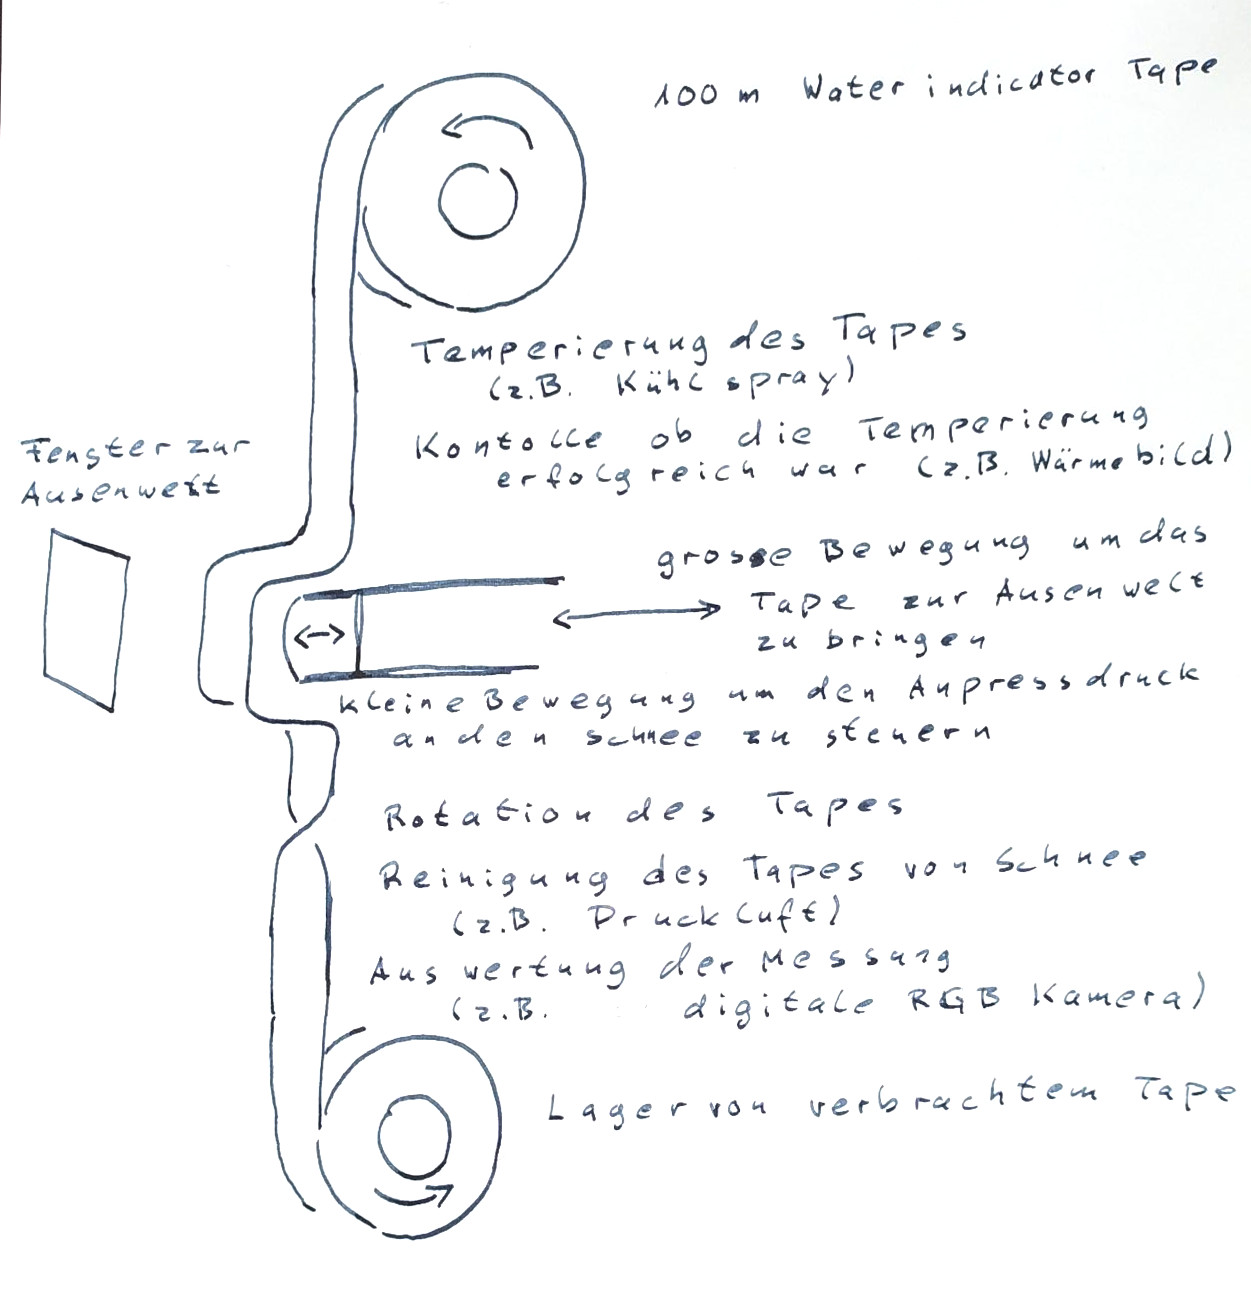
\includegraphics[width=0.8\textwidth]{Bilder/KonzeptAut.jpeg}
    \caption{Ablauf einer automatischen Messung}
    \label{fig:AutMess}
\end{figure}
